% !TEX program = xelatex
% !BIB program = bibtex

\documentclass[UTF8,12pt,a4paper]{article}
\usepackage{ctex}

% layout
\usepackage[left=2.5cm,right=2.5cm]{geometry}
\usepackage{paralist}     % for compactitem environment
\usepackage{indentfirst}  % ident the first paragraph
\linespread{1.25}
% \makeatletter
% \def\@seccntformat#1{%
%   \expandafter\ifx\csname c@#1\endcsname\c@section
%   Section \thesection:
%   \else
%   \csname the#1\endcsname\quad
%   \fi}
% \makeatother
 
% page headings
\usepackage{fancyhdr}
\setlength{\headheight}{15.2pt}
\pagestyle{fancy}
\lhead{\leftmark}
\rhead{M201873026 Yilong Liu}
\cfoot{\thepage}
% \makeatletter
% \let\headauthor\@author
% \makeatother

% url/ref
\usepackage{hyperref}
\hypersetup{
  colorlinks,
  citecolor=black,
  filecolor=black,
  linkcolor=black,
  urlcolor=black,
  pdfauthor={Yilong Liu},
  pdftitle={Graph Processing: state-of-the-art and research challenges}
}

% vertical centering title page
\usepackage{titling}
\renewcommand\maketitlehooka{\null\mbox{}\vfill}
\renewcommand\maketitlehookd{\vfill\null}

% table of contents
\usepackage{tocloft}
\renewcommand\cftsecfont{\normalfont}
\renewcommand\cftsecpagefont{\normalfont}
\renewcommand{\cftsecleader}{\cftdotfill{\cftsecdotsep}}
\renewcommand\cftsecdotsep{\cftdot}
\renewcommand\cftsubsecdotsep{\cftdot}
\renewcommand\cftsubsubsecdotsep{\cftdot}
\renewcommand{\contentsname}{\hfill\bfseries\Large Contents\hfill}   
\setlength{\cftbeforesecskip}{10pt}
\setcounter{tocdepth}{2}

% figures
\usepackage{graphicx}
\graphicspath{figures/}
% \newcommand\figureht{\dimexpr
%   \textheight-3\baselineskip-\parskip-.2em-
%   \abovecaptionskip-\belowcaptionskip\relax}


% tables
\usepackage{caption} 
% \captionsetup[table]{skip=10pt}

% math, algorithms, code
\usepackage{amsmath,amssymb,url}
\usepackage{algorithm,algorithmicx,algpseudocode}
\usepackage{listings}

\lstset{
   extendedchars=true,
   basicstyle=\footnotesize\ttfamily,
   showstringspaces=false,
   showspaces=false,
   numbers=left,
   numberstyle=\footnotesize,
   numbersep=9pt,
   tabsize=2,
   breaklines=true,
   showtabs=false,
   captionpos=b
}

% bibliography
\usepackage[super,square,comma,sort]{natbib} % for \citet and \citep
\renewcommand{\refname}{References}
% \begin{filecontents}{report.bib}
% \end{filecontents} 

% appendix
\usepackage{appendix}

\title{Survey \\ \bigskip \textbf{Graph Processing: state-of-the-art and research challenges}}
\author{Huazhong University of Science and Technology\\ School of Computer Science and Technology\\ M1801\\ M201873026\\ Yilong Liu}
\date{\today}

\begin{document}

\pagenumbering{gobble} % no page number
\maketitle
\newpage
% \null\thispagestyle{empty}
% \newpage

% \pagenumbering{roman}
% \section*{Abstract}\sectionmark{Abstract}
% \addcontentsline{toc}{section}{Abstract}
% \addcontentsline{toc}{section}{\protect\numberline{}Abstract}
% \newpage
% \pagenumbering{gobble} % no page number

\pagenumbering{roman}
\tableofcontents
\newpage
% \null\thispagestyle{empty}
% \newpage

\pagenumbering{arabic}

\section{Workload Characterization}
\begin{compactitem}
  \item Memory bandwidth is not fully utilized.
  there is the potential for significant performance improvement
  on graph codes with current off-chip memory systems.
  \item Graph codes exhibit substantial locality.
  Optimized graph codes experience a moderately
  high last-level cache (LLC) hit rate.
  \item Reorder buffer size limits achievable memory throughput.
  The relatively high LLC hit rate implies
  many instructions are executed for each LLC miss.
  These instructions fill the reorder buffer in the core,
  preventing future loads that will miss in the LLC from issuing early,
  resulting in unused memory bandwidth.
  \item Multithreading has limited potential for graph processing
  Likely achievable performance with only a modest number (2) of threads per core.
\end{compactitem}

Because message-passing is far less efficient than accessing memory in contemporary systems,
the efficiency of each core in a cluster is on average
one to two orders-of-magnitude lower than cores in shared-memory nodes.
This communication-bound behavior has led to
a single SSD Node is able to outperform a medium-sized cluster~\cite{DBLP:conf/osdi/KyrolaBG12}.

Graph algorithms have their scaling hampered by
load imbalance, synchronization overheads, and non-uniform memory access (NUMA) penalties.
Different input graph sizes and topologies can lead to
very different conclusions for algorithms and architectures.

References from~\cite{DBLP:conf/iiswc/BeamerAP15}~\cite{DBLP:conf/usenix/MalicevicLZ17}.

\subsection{Graph Shape}
Graphs can be divided into two broad categories: meshes and social networks.
Meshes (such as road maps or the finiteelement mesh of a simulated car body)
usually have a high diameter
and a degree distribution that is both bounded and low.
social networks have a low diameter (``small-world'')
and a power-law degree distribution (``scale-free'').

In a small-world graph, most nodes are not neighbors of one another,
but most nodes can be reached from every other by a small number of hops.
A scalefree graph has a degree distribution
that follows a power law, at least asymptotically.
The small-world property makes them difficult to partition,
the scale-free property difficult to load balance a parallel execution.

Uniform graph is low diameter, like a social network,
but its degree distribution is normal rather than a power law.
Uniform represents the most adversarial graph,
as by design it has no locality,
it serves to act as lower bound on performance.

\subsection{Locality Benchmark}
No executions sustain a high IPC and a high memory bandwidth
(MLP, memory-level parallelism).
(\textbf{tradeoff} between \textbf{computation} and \textbf{communication})
A processor can only execute instructions at a high rate
if it rarely waits on memory, and hence consumes little memory bandwidth.
Some executions are actually in the worst lower-left quadrant,
where they use little memory bandwidth, but their compute throughput is also low,
presumably due to \textbf{memory latency}.
MLP ($memory bandwidth \times memory latency$) $\propto$ MPKI (misses per kilo-instructions).

TLB misses are only measurably detrimental when
at least a moderate amount of memory bandwidth is utilized.
Maximum bandwidth obtained with the larger array is substantially
reduced due to increases in TLB refill time (THP is useful to MLP)
(confirmed by performance counters).

If the processor is already achieving moderate memory bandwidth utilization,
performance is insensitive to the branch misprediction rate.
When the processor is not memory-bound,
frequent branch mispredictions will hurt performance.

Lower cache misses, lower memory bandwidth.
Higher degress and scale-free graphs has lower cache misses.

With more cores, this NUMA penalty is reduced,
and for executions that use less memory bandwidth,
the NUMA penalty is reduced further.
Moving computation is better than moving data
when optimizing graph processing for NUMA.

Multithreading also has the potential to introduce new performance challenges.
More threads increase parallelism, which in turn can worsen the damage
caused by \textbf{load imbalances} and \textbf{synchronization overheads}.
If the workload of the two threads is heterogenous it is possible
for an SMT core to exceed MLP/IPM model.
One thread could generate most of the cache misses
sustaining a high effective MLP
while the other thread (unencumbered by cache misses)
could execute instructions quickly to increase IPM.

Many techniques can improve performance,
but all of them will have quickly diminishing returns,
so greatly improving performance will require a multifaceted approach.
\subsubsection{Locality Tips}
\begin{compactitem}
  \item To ensure consistency across runs,
  disable Turbo Boost (dynamic voltage and frequency scaling)
  \item To generate more MLP,
  add more parallel pointer chases to the same thread
\end{compactitem}

\subsection{Graph Algorithms}
Differ in \# of active vertices per iteration:
\begin{compactitem}
  \item only a subset active: BFS (vertex-centric + CSR/CSC)
  \item entire graph active: Pagerank, SpMV ...
\end{compactitem}

\subsection{Graph Representation}
\begin{compactitem}
  \item adjacency lists: dynamic allocation/count sort/radix sort
  \item CSR/CSC
\end{compactitem}
\subsubsection{CSR/CSC}
CSR 行压缩使得顶点的出边被连续存储, CSC 列压缩使得顶点的入边被连续存储,
若仅使用行压缩, 则可以连续地访问顶点的出边而需要随机访问顶点的入边.
若同时使用行压缩和列压缩, 则图中所有的边将被存储两份,
当修改边的值时, 存在数据同步的问题.

\subsection{Processing Model}
Vertex-centric paradigm has expressive potentials
to easily represent various kinds of graph algorithms,
and the high parallelism in the grain of vertex.
However, in the vertex-centric paradigm,
there can be random accesses to edges,
resulting in potentially heavy memory access overhead.

Edge-centric paradigm is lack of flexible scheduling potential
in contrast to the vertex-centric one.
Almost all of edges have to be processed multiple times
to complete the whole process.
This paradigm may also lead to
a large number of random accesses to vertices.

\subsection{Message Passing}
\subsubsection{Push}
Push information to neighbors, write to state of others:
Good when few vertices are active, but Needs locks.
\subsubsection{Pull}
Pull information from neighbors, write to own state:
Good when many vertices are active, Locks can be avoided.
\begin{figure}
  \begin{small}
    \begin{center}
      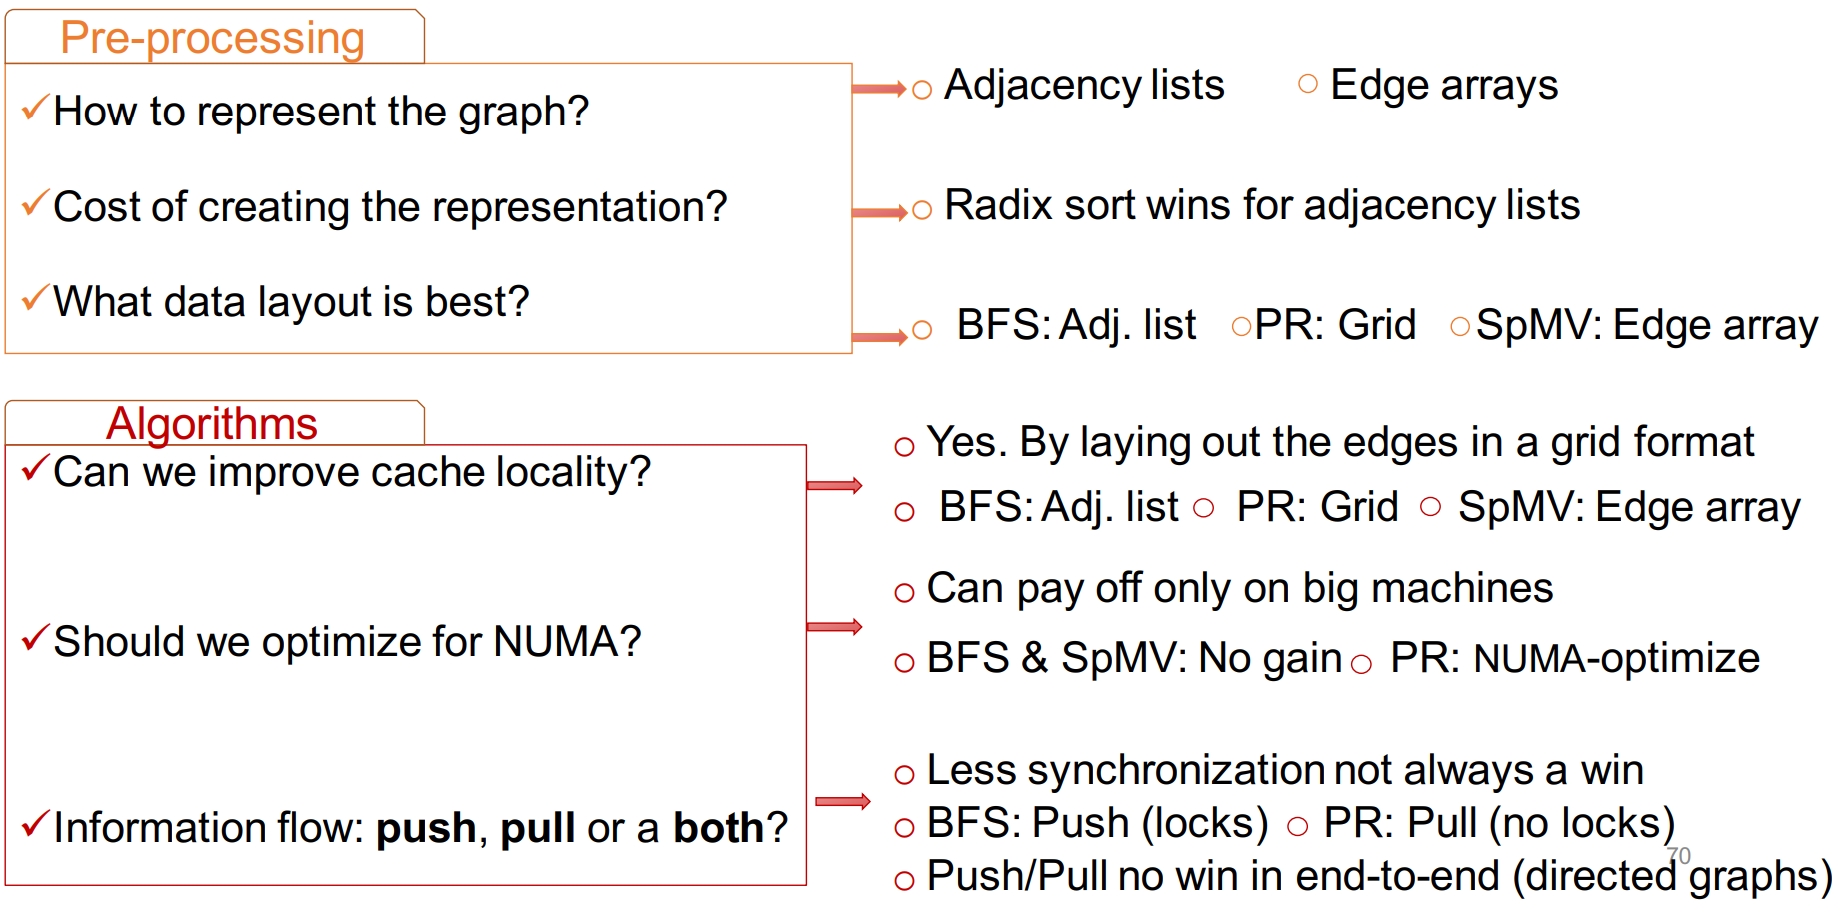
\includegraphics[width=0.95\textwidth]{figures/graph_atc17_everythinggraph1}
    \end{center}
    \caption{Everything in Graph Processing~\cite{DBLP:conf/usenix/MalicevicLZ17}}
    \label{fig:everythinggraph1}
  \end{small}
\end{figure}
\begin{figure}
  \begin{small}
    \begin{center}
      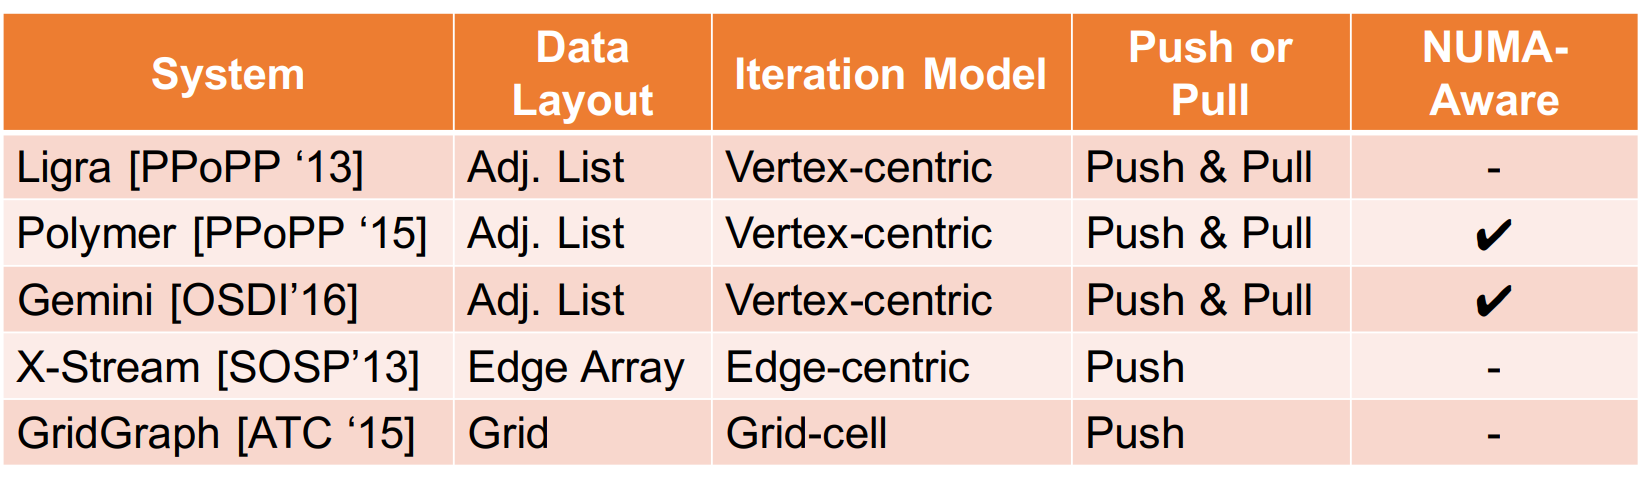
\includegraphics[width=0.95\textwidth]{figures/graph_atc17_everythinggraph2}
    \end{center}
    \caption{Everything in Graph Processing System~\cite{DBLP:conf/usenix/MalicevicLZ17}}
    \label{fig:everythinggraph2}
  \end{small}
\end{figure}
\clearpage

\section{Graph Processing System}
图计算框架核心问题:
\begin{compactitem}
  \item 任务划分与映射机制: TLP/DLP + mapping (programming/compiler/runtime)
  \item 独立/统一内存地址空间
  \item 内存数据组织: 图数据结构(CSR/Grid)/NUMA 数据放置
  \item 并发控制与同步机制: BSP/Pull/Push/Dataflow
\end{compactitem}

图计算特点:
\begin{compactitem}
  \item 规模巨大
  \item 局部性差
  \item 耦合性强
  \item 数据可能动态变化
  \item 计算过程频繁迭代
  \item intensive data access:
  most of the operations in graph processing are related to data accesses
  \item irregular computation: poor workloads balance (power-law distribution)
  \item poor locality: high memory access overhead
  \item high data dependency: make it difficult to explore the parallelism 
\end{compactitem}

高能效的大规模图计算
系统本质上主要包含两方面挑战:
处理引擎, 如何高效地处理图数据;
底层存储, 如何高效地存储和快速地访问图数据.

控制流体系结构为主的现代计算机系统带来了访存局部性差, 并行流水执行效率低,
内外存通道有限以及同步的扩展性差等一系列挑战.
在内存带宽不足的情况下, 内存带宽是图数据处理任务的主要瓶颈.
随着内存性能的逐渐提高和各种新型内存技术的出现,
图计算本身的调度和同步开销将逐渐成为新的主要性能瓶颈.
由于受到传统控制流体系结构的限制,
现有方案在优化手段上较为单一而难以进一步提高图计算系统的性能.
综上所述,为实现基于异构系统的图计算的``高性能, 可扩展, 易编程''目标,
学术界和工业界还需要在异构平台图计算协同调度, 高效的数据管理机制,
高度抽象且易用的异构图编程框架等关键技术方面进行进一步的研究和突破.

\subsection{图计算系统分类}
按架构分类:
\begin{compactitem}
  \item 单机图计算系统: 指在单机上利用多核CPU, 大内存和多线程并行等进行大规模图计算.
  这类系统通过减少磁盘随机写操作, 避免高昂的通信开销,
  采用并行化技术来充分挖掘多核计算资源来处理大规模图数据,
  在图的规模不是很大的情况下, 能在可接受的时间范围内完成任务,
  达到与分布式大规模图计算系统相当的时间性能.
  已有的主要单机图计算系统包括: GraphChi~\cite{DBLP:conf/osdi/KyrolaBG12},
  X-Stream~\cite{DBLP:conf/sosp/RoyMZ13},
  TurboGraph~\cite{DBLP:conf/kdd/HanLPL0KY13},
  Ligra~\cite{DBLP:conf/ppopp/ShunB13},
  Galois~\cite{DBLP:conf/sosp/NguyenLP13},
  FlashGraph~\cite{DBLP:conf/fast/ZhengMBVPS15},
  GridGraph~\cite{DBLP:conf/usenix/ZhuHC15},
  PathGraph~\cite{DBLP:journals/tpds/YuanXLJ16}.
  \item 分布式图计算系统: Pregel~\cite{DBLP:conf/sigmod/MalewiczABDHLC10},
  GraphLab~\cite{DBLP:journals/pvldb/LowGKBGH12},
  PowerGraph~\cite{DBLP:conf/osdi/GonzalezLGBG12},
  Polymer~\cite{DBLP:conf/ppopp/ZhangCC15},
  Gemini~\cite{DBLP:conf/osdi/ZhuCZM16}.
\end{compactitem}

按计算模型分类:
\begin{compactitem}
  \item BSP
  \item 以顶点为中心的 GAS, 可以 CSR/CSC 压缩, 可以快速地遍历顶点的边 (高效 Gather), 不需要原子操作
  数据预处理时, 对边集进行排序消耗可观; 
  需要随机访问邻接节点, 当邻接节点不在内存时会产生磁盘随机访问
  \item 以边为中心的 GAS. 边集 E 远大于顶点集 V, 可以降低通信开销.
  虽然可以处理无序边, 但无法压缩;
  若多条边访问同一节点, 需要原子操作
  \item 以顶点为中心 GAS 计算模式适用于度高的顶点 (特别对于 Gather, 可以大量减少访存),
  而以边为中心 GAS 计算模式适用于度低的顶点
\end{compactitem}


\subsection{GraphChi}
GraphChi~\cite{DBLP:conf/osdi/KyrolaBG12}具有以下特点:
\begin{compactitem}
  \item 以顶点为中心的 GAS 模型核外单机图计算系统
  \item 将连续顶点集划分为 P 个 interval, 每个 interval 对应一个 shard,
  存储着所有入边 (即一个 shard 对应一个子图, 边以源点排序保存)
  \item 利用 PSW (parallel sliding window) 每次访问一个 shard 中所有边与其他 shards 中的出边
  \item `input --(create shards)--> shards --(run algorithm)--> output`
  \item 尽管需要进行预处理 (创建 shards, 排序等), 但对于需要长期运行的系统而言, 这仅仅需要进行非常少的次数 (one time cost)
  \item 通过 CSR + PSW 结合, 使得 Gather 阶段顺序访问节点的入边 (遍历所属 interval 的整个 shard)
  Scatter 阶段顺序访问节点的出边 (由于 shard 内部按源点顺序排列, 所以只需遍历其他 interval 的部分 shard)
\end{compactitem}
\subsubsection{Shortcoming}
\begin{compactitem}
  \item 构建 shard 是需要对边按源顶点排序,这样耗费了大量的预处理时间,PWS 对计算密集型的算法更有利
  \item 另外在构建子图时出现大量的随机访存现象,通过顺序地更新子图内有共享边顶点来避免数据争用问题
  \item GraphChi 计算过程和磁盘 I/O 访问之间串行执行, 可以通过重叠这两部分进一步提升性能
\end{compactitem}

\subsection{X-Stream}
X-Stream~\cite{DBLP:conf/sosp/RoyMZ13}具有以下特点:
\begin{compactitem}
  \item 以边为中心的 GAS 模型核外单机图计算系统
  \item 将边划分为多个流式分区 (分区内无需排序), 顺序化地访问每个分区中的所有边
  \item 随机访问快速存储介质中的数据 (如顶点数据), 顺序访问慢速存储介质中的数据 (如边数据)
  \item `input --(run algorithm)--> output`
  \item 没有预处理开销
\end{compactitem}
\subsubsection{Shortcoming}
\begin{compactitem}
  \item X-Stream在计算过程中,每轮迭代产生的更新集非常庞大,接近于边的数量级
  \item 需要对更新集中的边进行 shuffle 操作
  \item 缺乏选择调度机制,产生了大量的无用计算
\end{compactitem}

\subsection{TurboGraph}
TurboGraph~\cite{DBLP:conf/kdd/HanLPL0KY13}设计了一种页结构,
只需加载部分图结构,基于 pin-and-slide 模型, 设计了两种不同类型的线程,
即执行线程和回调线程, 且执行线程和 I/O 回调线程可以并行处理,
从而提高了线程间的并行度, 避免了迭代过程中大量中间结果访问磁盘开销,
并利用固态硬盘实现磁盘读写和计算的并行化, 提高了图计算的整体性能。

\subsection{Ligra}
Ligra~\cite{DBLP:conf/ppopp/ShunB13} is built on
the abstractions of edge maps and vertex maps.
When applying these map functions,
Ligra uses heuristics to determine in
which direction to apply them (push or pull)
and what data structures to use (sparse or dense).
These optimizations make Ligra especially well suited for low-diameter graphs.

\subsection{Galois}
Galois~\cite{DBLP:conf/sosp/NguyenLP13}
are designed to handle irregular fine-grained task parallelism.
Algorithms implemented in Galois
are free to use autonomous scheduling (no synchronization barriers),
which reduce the synchronization needed for high-diameter graphs.

\subsection{FlashGraph}
FlashGraph~\cite{DBLP:conf/fast/ZhengMBVPS15}
是一个能在固态硬盘阵列上处理具有万亿节点的半外存的单机图计算系统.

\subsection{GridGraph}
\subsubsection{Motivation}
GridGraph~\cite{DBLP:conf/usenix/ZhuHC15} 是以边为中心的核外单机图计算系统,
基于 X-stream, 能否进行实时更新, 从而进一步减少 I/O 开销:
将 scatter 阶段的顺序化写入与 gather 阶段的顺序化读出进行一定程度上地合并,
即合并 updates 操作
\subsubsection{Solution}
\begin{compactitem}
  \item 在进行流式分区时, 保证 scatter 阶段的源顶点与 gather 阶段的目的顶点的局部性 (使其位于同一个 streaming partion)
  \item 利用 Grid Representation 可以达到这一目的:
  两级结构的分区 (2-level hierarchical partitioning) + 双滑动窗口 (Dual sliding windows)
\end{compactitem}
\subsubsection{Grid Representation}
\begin{compactitem}
  \item 将顶点划分为 P 个相等的 chunks
  \item 将边划分为 P x P 个 blocks: 边源顶点所在的chunk决定其在网格中的行,边目的顶点所在的chunk决定其在网格中的列
\end{compactitem}
第 n 行中的边的源顶点应为 chunk-n 中的顶点,
第 n 列中的边的目的顶点应为 chunk-n 中的顶点: 第 (m, n) 个 block 中的边的源顶点应为 chunk-m 中的顶点,
目的顶点应为 chunk-n 中的顶点
\subsubsection{Dual Sliding Windows}
\begin{compactitem}
  \item 以列优先的顺序逐块遍历 edge blocks (自上至下, 自左至右)
  \item 以列优先的顺序遍历时, 可以减少写带宽 (gather 阶段的 updates)
\end{compactitem}
\subsubsection{Selective Scheduling}
跳过不具有活跃边的 blocks, 减少不必要的 I/O
\subsubsection{2-Level Hierarchical Partitioning}
将每个 Block 进行进一步的 Grid 划分
\subsubsection{GridGraph Shortcoming}
\begin{compactitem}
  \item 折线式的边 block 遍历策略不能达到最大化的Cache/Memory命中率
\end{compactitem}

\subsection{PathGraph}
PathGraph~\cite{DBLP:journals/tpds/YuanXLJ16}
是一个采用路径中心计算模型的单机图计算系统, 通过构建前向边遍历树和后向边遍历树,
将图算法的每次迭代计算分解为沿前向边遍历树更新数据和沿后向边遍历树收集消息的两步操作.

\subsection{Pregel}
Pregel~\cite{DBLP:conf/sigmod/MalewiczABDHLC10}
是一种基于 BSP 模型, 以顶点为中心的分布式图处理系统.
BSP 模型是一种基于消息通信的并行计算模型,
计算由一系列称为超步 (Superstep) 的通过全局同步分开的计算步骤组成,
采用块间同步处理, 块内异步并行的计算.
并行任务按照超步组织, 接收来自上一个超步的消息, 执行本地计算并发送消息给下一个超步.
每个超步包含了三个过程:
\begin{compactitem}
  \item 本地计算: 每个工作节点读取其本地数据异步地执行计算
  \item 消息通信: 
  每个参与计算的工作节点将消息发给与之相连的其它工作节点以相互交换所需的数据
  \item 路障同步: 用于数据的全局同步,即块间同步,
  每个工作节点在更新完自身的消息缓存并确一个超步
\end{compactitem}
由于超步中每个节点上的本地计算的执行时间不等, 进度不统一, 
全局路障同步将会导致大量节点进入等待状态, 形成快等慢的局面,
进而产生``木桶效应'', 造成计算资源的浪费.
且这种方式的工作节点间的通信量较多, 也会加大时间开销.
基于 BSP 模型的分布式图计算系统在处理具有幂率分布的图时效率较低.

\subsection{GraphLab}
GraphLab~\cite{DBLP:journals/pvldb/LowGKBGH12}
是一种基于 GAS 模型的分布式图处理系统,
对 BSP 模型进行进一步细化, 提高并行度.
其采用异步执行模式, 即可以使用相邻顶点或边中存储的最新数据来更新当前顶点状态.
采用异步模式将不可避免的面临数据竞争问题, 例如:
正在处理顶点 V 的函数需要访问邻接顶点,
而邻接顶点此刻正在更新其状态;
各自处理不同顶点的多个函数可能出现同时写共享数据.
为了保证顺序一致性, 即所有的并行执行操作都有一个等价的顺序执行操作序列与之对应,
从而确保并行执行与顺序执行都产生相同的结果.
这就要求存在数据竞争的顶点之间需要按照一定的顺序串行执行,
GraphLab 利用顶点着色、分布式锁等机制来确保存在竞态的顶点被顺序执行,
而不存在竞态的顶点能够被并行执行.
GraphLab 将需要被处理的顶点置入集合 T, 从集合 T 中取出顶点进行处理,
同时将 Receiver 从 T 中移出, 需要被处理的顶点又被动态地加入到集合 T 中.
当集合 T 为空时, 执行结束.

\subsection{PowerGraph}
PowerGraph~\cite{DBLP:conf/osdi/GonzalezLGBG12}
基于 GraphLab, 利用``长尾''现象来优化子图划分,
尽可能地实现负载均衡和最小化通信与存储开销.
其提出了顶点分割方案, 即对于度较高的顶点进行分割,
分割开来的边被放置到不同的节点, 每个节点只需要维护被分割的顶点的镜像即可.

GAS 模型具有更好的灵活性, 适应大多数图算法,
并发任务间不需要数据同步过程, 每个并发任务在任意时刻都可以对全局参数进行读和更新,
这提升了计算资源的利用率和整体任务的执行效率.
但是仍有一定的缺陷: 假设某些任务由于硬件故障或者机器负载高,
在迭代次数上严重滞后于其它任务, 则有可能使正确性无法得到完全保证.

\subsection{Polymer}
Polymer~\cite{DBLP:conf/ppopp/ZhangCC15}.

\subsection{Gemini}
Gemini~\cite{DBLP:conf/osdi/ZhuCZM16} major optimizations:
\begin{compactitem}
  \item efficiency: adaptive push-/pull-style computation
  \item efficiency: hierarchical chunk-based	partitioning
  \item scalability: locality-aware	chunking
  \item scalability: chunk-based work-stealing
\end{compactitem}

Gemini organizes outgoing edges in the Compressed Sparse Row (CSR)
and incoming ones in the Compressed Sparse Column (CSC) format.

Sparse mode for push operations, dense mode for pull operations (locks-free).
When it comes to distributed push/pull mode,
masters	push message to mirrors, who update	their	local	neighbors.
mirrors	pull updates from	neighbors, then	message	remote masters.

Gemini considers both	vertex and edge:
\begin{compactitem}
  \item Edge:	the	amount of	work to	be processed
  \item Vertex:	the	processing speed of	work (locality)
  \item Hybrid metric: $\alpha \cdot \vert V_i \vert + \vert E_i \vert$
\end{compactitem}

Divide vertex	set into contiguous chunks.
Chunk-based partitioning preserves locality.
It's affordable	for preprocessing	when vertices	unordered.
Per-node partition, per-socket partition, per-core work chunk
(work partitioning within socket, mini-chunk for work-stealing).
Gemini design a co-scheduling mechanism to
overlap computation and inter-node communication tasks.
\clearpage

\section{FPGA}
FPGA in Data Center~\cite{DBLP:conf/isca/PutnamCCCCDEFGGHHHHKLLPPSTXB14}.

\begin{compactitem}
  \item cpu 通用
  \item gpu 高吞吐量
  \item fpga 低延迟
\end{compactitem}

FPGA 比 CPU 和 GPU 能效高, 体系结构上的根本优势是无指令, 无需共享内存.
缺少指令同时是 FPGA 的优势和软肋. 每做一点不同的事情, 就要占用一定的 FPGA 逻辑资源.
如果要做的事情复杂或重复性不强, 就会占用大量的逻辑资源, 其中的大部分处于闲置状态.
不管通信还是机器学习, 加密解密, 算法都是很复杂的,
如果试图用 FPGA 完全取代 CPU, 势必会带来 FPGA 逻辑资源极大的浪费, 也会提高 FPGA 程序的开发成本.
更实用的做法是 FPGA 和 CPU 协同工作, 局部性和重复性强的归 FPGA, 复杂的归 CPU.

CPU 可以通过 PCIe 总线与 FPGA 直接通信, 无需通过基于共享内存(FPGA 片上内存)的批处理模式.
通过 OpenCL 写 DRAM, 启动 kernel, 读 DRAM 一个来回, 需要 1.8 毫秒.
而通过 PCIe DMA 来通信, 却只要 1~2 微秒.

在数据中心里 FPGA 的主要优势是稳定又极低的延迟, 适用于流式的计算密集型任务 (低延迟) 和通信密集型任务.
FPGA 定义为通信的\textbf{大管家}, 不管是服务器跟服务器之间的通信, 虚拟机跟虚拟机之间的通信,
进程跟进程之间的通信, CPU 跟存储设备之间的通信, 都可以用 FPGA 来加速.
从第一代装满 FPGA 的专用服务器集群, 到第二代通过专网连接的 FPGA 加速卡集群 (8x6),
到目前复用数据中心网络的大规模 FPGA 云 (FPGA 部署在网卡和交换机之间).

Massive parallelism can be easily achieved when these resources are in good use.
For improving the locality of vertices on the BRAM,
fine grained partitioning and dedicated data placement strategies
are needed to increase the reuse rate of vertices on the BRAM.

Shortcoming:
\begin{compactitem}
  \item limited resources (BRAM, PLE)
  \item limited frequency
\end{compactitem}


\subsection{Tesseract}
Tesseract~\cite{DBLP:conf/isca/AhnHYMC15}其是一个由 16 个立方构成的立方网络.
每个立方是一个混合内存立方体(HMC, Hybrid Memory Cube), 具有 512 GB/s 内部内存带宽.
每个混合内存立方体由 32 个垂直切片构成, 将每个垂直切片称为一个 vault, 多个 vault 间通过交叉开关网络连接.
每个 vault 包含一个 16 个块的 DRAM 分区, 一个专用内存控制和一个轻量级通用处理器.
Tesseract 具有 8 TB/s (16 x 512 GB/s) 内部内存带宽, 具有 16 x 32 = 512 个通用处理器.
在开始处理图数据前, 按照一定的划分规则将图数据划分为 512 个子图, 每个 vault 对应一个子图.

\subsection{EEAGAA}
EEAGAA~\cite{DBLP:conf/isca/OzdalYKAGBO16} 采用以顶点为中心计算模式,
并采用行压缩 (CSR) 格式来表示图数据, 在执行图算法时, 遵循 GAS 模型, 并支持异步执行模式.
其内部包括片上缓存、访存请求处理、活跃顶点列表管理、运行时管理部件、
信息收集计算部件、顶点状态更新计算部件、信息扩散计算部件和同步部件.

\subsection{Graphicionado}
Graphicionado~\cite{DBLP:conf/micro/HamWSSM16}
是一个采用以边为中心, 遵循同步执行模式的图计算加速器,
其指出当前的通用处理器不是进行图数据处理的理想平台,主要原因包
括:
\begin{compactitem}
  \item 访存粒度过大, 导致片外访存带宽被浪费.
  通用处理器从内存载入或存储数据的粒度是缓存行,
  一个缓存行的大小一般为 64 字节, 而图算法访问数据的粒度一般为 4 字节
  \item 低效的片上缓存使用. 通用处理器不能有效地将局部性高的数据存储于片上缓存中
  \item 不匹配的执行粒度. 通用处理器使用指令来完成计算和访存操作,
  对很多图算法, 绝大部分指令主要用于供给数据和移动数据, 其能效差.
\end{compactitem}
其建立了片上存储用于存储顶点信息, 同时降低访存粒度, 设计硬件专用流水线进行图计算.

\subsection{ForeGraph}
ForeGraph~\cite{DBLP:conf/fpga/DaiHCXWY17}
adopts \textbf{Grid} data layout into distributed FPGA boards.

\subsection{FabGraph}
FabGraph~\cite{DBLP:conf/fpga/ShaoLHL019}
adopts two-level vertex caching,
L1 vertex caches attached to pipeline sets,
L2 vertex caches as shared vertex buffer.
All vertex caches use BRAM.
FabGraph use 2 pipeline sets to overlap
communication and computation,
enhancing bandwidth of graph progressing.
FabGraph only needs to slide the window
to cover the upper-triangular part or lowertriangular part of the grid,
reduceing data transmission.

\clearpage

\section{DRAM}
Core (核) 代表一个独立的 CPU, Socket (颗) 本意是插槽,
代表一个主板上的芯片, 多核架构就是在一个芯片上放多个处理器,
2颗4核, 代表主板上有 2 个芯片插槽, 每个芯片上存在 4 个 CPU, 所以有 8 个物理 CPU,
如果存在超线程, 还可能多出 8 个逻辑 CPU, 总共 16 个逻辑 CPU.
一个逻辑 CPU(LCPU)能运行一个进程或线程, 如果每核能执行 2 个或更多的线程,
那么一定使用了超线程技术, 否则每一核就只能运行一个线程或进程.

SRAM 容量太难做大, CPU 一半以上的面积都用来做 SRAM.
SRAM 面积越大, 速度就越慢.
SRAM 做到 GB 容量几乎是不可能完成的任务.

\subsection{Basis of DRAM}
\subsubsection{Terminology}
\begin{compactitem}
  \item RAS: Row Address Strobe (ACT Activate DRAM page/row Command)
  \item CAS: Column Address Strobe (READ Command)
  \item DDR: Double-Data Rate transfers data
  on both rising and falling edge of the clock
  \item Channel: 一组数据信号线、对应几个槽位、对应几根内存条称为一个 channel
  \item Bank: read out all words in parallel, 一个 bank 包含 N 个 DRAM Subarray (N*row*col*1bit)
  \item DIMM: Dual Inline Memory Module 双通道内存
  \item channel>DIMM>rank>chip>bank>row/column
\end{compactitem}
\subsubsection{Address Mapping Scheme}
如表~\ref{tab:dram_address_mapping}所示,
$\text{Memory Capacity} = K*L*B*R*C*V$,
$N = CV/Z$, $CV = NZ$.
采用 open page (keep page in DRAM row buffer) 时,
映射为 k:l:r:b:n:z (可扩展) /r:l:b:n:k:z (高并行) (n 也等于 column, z 也等于 offset).
采用 close page (immediately close page in DRAM row buffer) 时,
映射为 k:l:r:n:b:z/r:n:l:b:k:z.
Accessing different rows from one bank is slowest.
\begin{table}
  \begin{small}
    \caption{DRAM Address Mapping Parameters}
    \label{tab:dram_address_mapping}
    \begin{center}
      \begin{tabular}[c]{l|l}
        \hline
        \multicolumn{1}{c|}{\textbf{Symbol}} & 
        \multicolumn{1}{c}{\textbf{Description}} \\
        \hline
        K & \# of channels in system \\
        L & \# of ranks per channel \\
        B & \# of banks per rank \\
        R & \# of rows per bank \\
        C & \# of columns per row \\
        V & \# of bytes per column \\
        Z & \# of bytes per cache line \\
        N & \# of cache lines per row \\
        \hline
      \end{tabular}
    \end{center}
  \end{small}
\end{table}
\subsubsection{Delay Time}
一条访存指令发到内存控制器, 它的访存延时是存在不同的可能性:
\begin{compactitem}
  \item row buffer hit: 从 row buffer 到把数据放在数据总线上的时延,大约 20 ns
  \item empty row buffer: 从电容到 sense amplifier 再到 row buffer 的时序 + 从 row buffer 到数据总线时间,大约40ns
  \item row buffer conflict: 写回时延 + empty row buffer delay, 大约60ns
  \item CL: CAS Latency, 从 CAS 与读取命令发出到第一笔数据输出的这段时间 (READ -> data)
  \item tRCD: RAS 到 CAS 时延 (Active -> READ)
  \item 要切换另一行,要发 precharge 命令 (close page/row), 把数据写到 cell 里去.
  关闭一个行需要时间, 这个时间称为 tRP, 发送 PRE/PREA 命令后 tRP 时间才可以发 ACT 命令.
\end{compactitem}

\subsection{Memory Controller}
来自 CPU 的请求以执行顺序进入 transaction queue,
这些请求被转换为 DRAM 命令并放入 command queue.

\subsection{Landscape of DRAM-based memory}
\begin{table}
  \begin{small}
    \caption{Landspace of DRAM-based memory~\cite{DBLP:journals/cal/KimYM16}}
    \label{tab:memory_landscape}
    \begin{center}
      \begin{tabular}[c]{l|l}
        \hline
        \multicolumn{1}{c|}{\textbf{Segment}} & 
        \multicolumn{1}{c}{\textbf{DRAM Standards \& Architectures}} \\
        \hline
        Commodity & DDR3;DDR4 \\
        Low-Power & LPDDR3;LPDDR4 \\
        Graphics & GDDR5 \\
        Performance & eDRAM;RLDRAM3;WIO;WIO2;MCDRAM \\
        3D-Stakced & HBM;HMC;SBA/SSA;Staged Reads;RAIDR \\
        Academic & SALP/SARP;AL/TL-DRAM;RowClone;Half-DRAM;Row-Buffer Decoupling \\
        \hline
      \end{tabular}
    \end{center}
  \end{small}
\end{table}

\subsection{Simulator}
\subsubsection{DRAMSim2}
\begin{compactitem}
  \item AddressMapping.cpp: 物理地址到内存 (rank/bank/row/col/offset) 的映射关系
  \item TraceBasedSim.cpp: trace file (.trc) 相关代码
\end{compactitem}
\clearpage

\section{DragonGraph}

GPUs also face the drawbacks,
e.g., control and memory divergence,
load imbalance and global memory access overhead.

\subsection{Basic Infrastructure}
\begin{compactitem}
  \item Enhanced/Redundant CSR
  \item vertex-centric
  \item GAS (sync)
  \item push (locks) when few vertices discovered (early iterations),
  \item pull (no locks) when many vertices discovered (late iterations).
  \item no NUMA
  \item Verilog or Sdaccel
\end{compactitem}

\subsection{Grpah Kernels or Grpah Benckmarks}
\begin{compactitem}
  \item SSSP
  \item CC
  \item best-first search
  \item uniform-cost search
  \item greedy-search
  \item A*
\end{compactitem}

\subsection{Key Optimization}
Different types of locality:
hierarchical networks, distributed,
shared and local caches, local and non-local memory,
and various cache-coherence effects.
\begin{compactitem}
  \item improve poor locality
  \item use of a bitmap to mark the vertices during the visit
  \item FastForward queue (PPoPP'08)
  \item use of batching when inserting and removing
  from the inter-socket communication channel to amortize the locking overhead
  \item software prefetching
  \item cut off NUMA communication
  \item parallelism: dataflow (pipelined Multiple Instructions Single Data (MISD) model)
  \item MLP: HBM
  \item coalescing multiple into single one
  \item reshape cache hierachy
  \item locality-aware vertices buffer
  \item enhanced CSR/CSC
  \item work stealing
  \item overlap communication and computation with multiple pipelines/boards
\end{compactitem}

\subparagraph{ILP}
Vertex dependencies of graph can stall the pipelines
and decrease the instruction level parallelism.
How to reduce the impact arising from data dependencies
remains an open problem for increasing the number of Instructions per Cycle (IPC).

\subparagraph{MLP}
Multi-bank, multi-port, optimizied memory access.
The memory bandwidth utilization here means
the valid values ratio per transfer.
Random accesses in graph processing usually cause
low ratio of valid values and result in much wasted bandwidth.
Improving the memory bandwidth utilization can reduce the total number of memory accesses.

\subparagraph{Asynchronous}
Asynchronous mode requires tremendous efforts
to implement on graph accelerators for the sophisticated hardware design.

\section{Graph Survey Template}
\begin{compactitem}
  \item data presentation/layout
  \item data ordering: index-aware/degree-aware/conflict-aware
  \item data partition: source-oriented/destination-oriented
  \item data manipulation
  \item open source
  \item programming model
  \item partioning
  \item static and dynamic graphs
  \item batch and streaming
  \item algorithms
  \item community activity
  \item users
  \item books 
  \item distinction points
\end{compactitem}
\clearpage

\bibliographystyle{unsrt}
\bibliography{bibs/graph}
\addcontentsline{toc}{section}{References}
\newpage

\end{document}
